% Options for packages loaded elsewhere
\PassOptionsToPackage{unicode}{hyperref}
\PassOptionsToPackage{hyphens}{url}
%
\documentclass[
  man,floatsintext]{apa6}
\usepackage{amsmath,amssymb}
\usepackage{lmodern}
\usepackage{iftex}
\ifPDFTeX
  \usepackage[T1]{fontenc}
  \usepackage[utf8]{inputenc}
  \usepackage{textcomp} % provide euro and other symbols
\else % if luatex or xetex
  \usepackage{unicode-math}
  \defaultfontfeatures{Scale=MatchLowercase}
  \defaultfontfeatures[\rmfamily]{Ligatures=TeX,Scale=1}
\fi
% Use upquote if available, for straight quotes in verbatim environments
\IfFileExists{upquote.sty}{\usepackage{upquote}}{}
\IfFileExists{microtype.sty}{% use microtype if available
  \usepackage[]{microtype}
  \UseMicrotypeSet[protrusion]{basicmath} % disable protrusion for tt fonts
}{}
\makeatletter
\@ifundefined{KOMAClassName}{% if non-KOMA class
  \IfFileExists{parskip.sty}{%
    \usepackage{parskip}
  }{% else
    \setlength{\parindent}{0pt}
    \setlength{\parskip}{6pt plus 2pt minus 1pt}}
}{% if KOMA class
  \KOMAoptions{parskip=half}}
\makeatother
\usepackage{xcolor}
\IfFileExists{xurl.sty}{\usepackage{xurl}}{} % add URL line breaks if available
\IfFileExists{bookmark.sty}{\usepackage{bookmark}}{\usepackage{hyperref}}
\hypersetup{
  pdftitle={Try and forget this image: The role of stimulus duration in directed forgetting for natural scenes},
  pdfauthor={Patrick Ihejirika1},
  pdflang={en-EN},
  pdfkeywords={Directed Forgetting, Picture Memory},
  hidelinks,
  pdfcreator={LaTeX via pandoc}}
\urlstyle{same} % disable monospaced font for URLs
\usepackage{graphicx}
\makeatletter
\def\maxwidth{\ifdim\Gin@nat@width>\linewidth\linewidth\else\Gin@nat@width\fi}
\def\maxheight{\ifdim\Gin@nat@height>\textheight\textheight\else\Gin@nat@height\fi}
\makeatother
% Scale images if necessary, so that they will not overflow the page
% margins by default, and it is still possible to overwrite the defaults
% using explicit options in \includegraphics[width, height, ...]{}
\setkeys{Gin}{width=\maxwidth,height=\maxheight,keepaspectratio}
% Set default figure placement to htbp
\makeatletter
\def\fps@figure{htbp}
\makeatother
\setlength{\emergencystretch}{3em} % prevent overfull lines
\providecommand{\tightlist}{%
  \setlength{\itemsep}{0pt}\setlength{\parskip}{0pt}}
\setcounter{secnumdepth}{-\maxdimen} % remove section numbering
% Make \paragraph and \subparagraph free-standing
\ifx\paragraph\undefined\else
  \let\oldparagraph\paragraph
  \renewcommand{\paragraph}[1]{\oldparagraph{#1}\mbox{}}
\fi
\ifx\subparagraph\undefined\else
  \let\oldsubparagraph\subparagraph
  \renewcommand{\subparagraph}[1]{\oldsubparagraph{#1}\mbox{}}
\fi
\newlength{\cslhangindent}
\setlength{\cslhangindent}{1.5em}
\newlength{\csllabelwidth}
\setlength{\csllabelwidth}{3em}
\newlength{\cslentryspacingunit} % times entry-spacing
\setlength{\cslentryspacingunit}{\parskip}
\newenvironment{CSLReferences}[2] % #1 hanging-ident, #2 entry spacing
 {% don't indent paragraphs
  \setlength{\parindent}{0pt}
  % turn on hanging indent if param 1 is 1
  \ifodd #1
  \let\oldpar\par
  \def\par{\hangindent=\cslhangindent\oldpar}
  \fi
  % set entry spacing
  \setlength{\parskip}{#2\cslentryspacingunit}
 }%
 {}
\usepackage{calc}
\newcommand{\CSLBlock}[1]{#1\hfill\break}
\newcommand{\CSLLeftMargin}[1]{\parbox[t]{\csllabelwidth}{#1}}
\newcommand{\CSLRightInline}[1]{\parbox[t]{\linewidth - \csllabelwidth}{#1}\break}
\newcommand{\CSLIndent}[1]{\hspace{\cslhangindent}#1}
\ifLuaTeX
\usepackage[bidi=basic]{babel}
\else
\usepackage[bidi=default]{babel}
\fi
\babelprovide[main,import]{english}
% get rid of language-specific shorthands (see #6817):
\let\LanguageShortHands\languageshorthands
\def\languageshorthands#1{}
% Manuscript styling
\usepackage{upgreek}
\captionsetup{font=singlespacing,justification=justified}

% Table formatting
\usepackage{longtable}
\usepackage{lscape}
% \usepackage[counterclockwise]{rotating}   % Landscape page setup for large tables
\usepackage{multirow}		% Table styling
\usepackage{tabularx}		% Control Column width
\usepackage[flushleft]{threeparttable}	% Allows for three part tables with a specified notes section
\usepackage{threeparttablex}            % Lets threeparttable work with longtable

% Create new environments so endfloat can handle them
% \newenvironment{ltable}
%   {\begin{landscape}\begin{center}\begin{threeparttable}}
%   {\end{threeparttable}\end{center}\end{landscape}}
\newenvironment{lltable}{\begin{landscape}\begin{center}\begin{ThreePartTable}}{\end{ThreePartTable}\end{center}\end{landscape}}

% Enables adjusting longtable caption width to table width
% Solution found at http://golatex.de/longtable-mit-caption-so-breit-wie-die-tabelle-t15767.html
\makeatletter
\newcommand\LastLTentrywidth{1em}
\newlength\longtablewidth
\setlength{\longtablewidth}{1in}
\newcommand{\getlongtablewidth}{\begingroup \ifcsname LT@\roman{LT@tables}\endcsname \global\longtablewidth=0pt \renewcommand{\LT@entry}[2]{\global\advance\longtablewidth by ##2\relax\gdef\LastLTentrywidth{##2}}\@nameuse{LT@\roman{LT@tables}} \fi \endgroup}

% \setlength{\parindent}{0.5in}
% \setlength{\parskip}{0pt plus 0pt minus 0pt}

% Overwrite redefinition of paragraph and subparagraph by the default LaTeX template
% See https://github.com/crsh/papaja/issues/292
\makeatletter
\renewcommand{\paragraph}{\@startsection{paragraph}{4}{\parindent}%
  {0\baselineskip \@plus 0.2ex \@minus 0.2ex}%
  {-1em}%
  {\normalfont\normalsize\bfseries\itshape\typesectitle}}

\renewcommand{\subparagraph}[1]{\@startsection{subparagraph}{5}{1em}%
  {0\baselineskip \@plus 0.2ex \@minus 0.2ex}%
  {-\z@\relax}%
  {\normalfont\normalsize\itshape\hspace{\parindent}{#1}\textit{\addperi}}{\relax}}
\makeatother

% \usepackage{etoolbox}
\makeatletter
\patchcmd{\HyOrg@maketitle}
  {\section{\normalfont\normalsize\abstractname}}
  {\section*{\normalfont\normalsize\abstractname}}
  {}{\typeout{Failed to patch abstract.}}
\patchcmd{\HyOrg@maketitle}
  {\section{\protect\normalfont{\@title}}}
  {\section*{\protect\normalfont{\@title}}}
  {}{\typeout{Failed to patch title.}}
\makeatother
\keywords{Directed Forgetting, Picture Memory}
\usepackage{csquotes}
\ifLuaTeX
  \usepackage{selnolig}  % disable illegal ligatures
\fi

\title{Try and forget this image: The role of stimulus duration in directed forgetting for natural scenes}
\author{Patrick Ihejirika\textsuperscript{1}}
\date{}


\shorttitle{Directed Forgetting}

\authornote{

An undergraduate honors thesis submitted to the Department of Psychology in partial fulfillment of the requirements for graduating with Departmental Honors. Advisor: Matthew Crump. This thesis should be computationally reproducible. All of the source code for the project is available at \url{https://www.crumplab.com/PatrickHonorsThesis/}

Correspondence concerning this article should be addressed to Patrick Ihejirika, Postal address. E-mail: \href{mailto:pihej121@gmail.com}{\nolinkurl{pihej121@gmail.com}}

}

\affiliation{\vspace{0.5cm}\textsuperscript{1} Brooklyn College of CUNY}

\abstract{
How useful would it be for you to selectively forget events that you choose to forget? Directed forgetting research is a tool used to investigate limitations on deliberate forgetting abilities. In a directed forgetting task people encode individual items and are instructed (cued) to either remember or forget them. A directed forgetting effect is observed when performance on a memory test is higher for remember-cued items than forget-cued items. Directed forgetting effects have been reproduced numerous times, and are commonly demonstrated in tasks using lists of words as the items to be remembered and forgotten (Epstein, 1969). Much less is known about directed forgetting for more memorable stimuli like images, pictures, and visual scenes. Ahmad, Tan \& Hockley showed that a weak directed forgetting effect can in fact be observed for image stimuli (2019). This poster investigates a general memory strength hypothesis of directed forgetting for pictures. According to this hypothesis, pictures are difficult to intentionally forget because they are encoded so well that attempts to forget the information are ineffective. I propose that weakening the encoding strength of images could allow intentional forgetting processes to operate more effectively, causing an increased directed forgetting effect. My experiments used the same general procedures as Ahmad, Tan, and Hockley (2019). In two experiments (n=45 each), I reduced encoding strength by manipulating stimulus duration during encoding (2000 ms {[}original amount{]}, 1000ms, or 500 ms per picture). I predicted that greater directed forgetting would be observed as stimulus duration decreased. I discuss the results of my two experiments in relation to the general memory strength hypothesis.
}



\begin{document}
\maketitle

\hypertarget{introduction}{%
\section{Introduction}\label{introduction}}

What is memory and how is it altered? Memory is often inaccurately defined as the ability to encode, store and retrieve information. A more accurate definition separates memory into two separate processes. Process one is characterized by remembering information and is defined as successfully encoding, storing and retrieving information. Process two is characterized by forgetting information. This definition allows for the conceptual introduction of intentionally controlling ones memory by selectively forgetting information details. The process by which information is forgotten can be explored using a directed forgetting procedure.

\hypertarget{what-is-directed-forgetting}{%
\subsection{What is Directed Forgetting?}\label{what-is-directed-forgetting}}

The directed forgetting procedure instructs participants to selectively remember or forget specific events and measures the accuracy with which participants are able to do so (for a review see, MacLeod, 1998). The design of a directed forgetting procedure consists of an encoding phase and a testing phase. The encoding phase presents participants with a series which is then followed by the presentation of instructional cues, directing participants to either remember or forget the previously presented stimulus. After the participants have been presented with all available stimuli, the testing phase begins. This testing phase then presents the same stimuli of the encoding phase against previously unseen stimuli, and tasks participants to accurately identify the stimulus presented in the encoding phase. Significantly lower accuracy in the recognition of forget-cued encoding stimuli is an indication of the presence of a phenomenon known as the directed forgetting effect.

\hypertarget{a-classic-demonstration-of-directed-forgetting}{%
\subsection{A classic demonstration of directed forgetting}\label{a-classic-demonstration-of-directed-forgetting}}

Bjork (1972) provides a description of traditional directed forgetting procedures. Generally, these procedures present participants with a series of items and cues. There are a number of ways to cue various item sets, including intraserial cuing, postinput cuing and pre-input cuing. The most common method of cuing item sets throughout traditional directed forgetting procedures is intraserial cuing. Intra-serial cuing sequentially presents participants with a set of items and directs them to either forget or remember said item using the cue's instruction. Though the item presented during such experiments may vary, traditional directed-forgetting procedures discussed throughout this paper use word stimuli as the presented items.
Traditional directed forgetting procedures also determine the presence and magnitude of a directed forgetting effect using either recognition or recall based testing conditions. Testing conditions which operationalize the directed forgetting effect as the accurate recall of ``Forget-cued'' stimuli do so by having participants recall as many wordage items as possible, without regard to the cue instructions. Previous research employing this recall-based directed forgetting procedure has identified a directed forgetting effect of 10-15\% for F-cued wordage stimuli, compared to the R-cued wordage stimuli (Weiner \& Reed, 1969). Testing conditions which operationalize the directed forgetting effect as the accurate recognition of ``Forget-cued'' stimuli do so by having participants identify as many previously seen wordage items as possible, without regard to the cue instructions.

\hypertarget{what-do-we-empirically-know-about-directed-forgetting}{%
\subsection{What do we empirically know about directed forgetting?}\label{what-do-we-empirically-know-about-directed-forgetting}}

MacLeod (1998) has identified 38 factors with the potential to influence the directed-forgetting effect. This paper will specifically focus on 4 of these 38 factors. These 4 factors include cue presentation time, stimulus presentation time, stimulus detail and stimulus type.

Wetzel (1977) used a directed forgetting procedure to explore the effects of cue duration on the participant recall accuracy of word stimuli. This exploration required the manipulation of both the stimuli presentation duration and the cue presentation duration during the encoding phase, creating two separate experimental conditions. These experimental conditions are known as the long delay condition and the short delay condition. The long-delay condition presents the word stimuli for a duration of 2, 4 or 8 seconds and the cue for a duration of 1 second, while the short-delay condition presents the word stimuli for a duration of 1 second and the cue for a duration of 2, 4 or 8 seconds. The result of this experiment indicates that short delay conditions, specifically conditions with short stimulus duration and long cue duration lead to an increased directed forgetting effect. These results serve as a motivation for the factorial manipulation of stimuli presentation duration within my experiment.

Ahmad, Tan, and Hockley (2019) used a directed forgetting procedure which explored the effects of stimuli details on accuracy of participant recognition of encoding phase stimuli. This was done through the introduction of novel testing conditions and exemplar conditions into the testing phase. Novel conditions present the same stimuli from the encoding phase against previously unseen stimuli, completely different to that of the encoding stimuli. Exemplar conditions present the same stimuli from the encoding phase against previously unseen stimuli similar to that of the encoding stimuli. Both conditions task participants to accurately identify the stimulus presented in the encoding phase. The results of this experiment indicate the existence of a significantly lower directed forgetting effect for novel testing conditions. This indication of significantly higher accuracy in participant recognition for novel testing conditions than exemplar testing conditions serves as a motivation for my experiment.

Traditional directed forgetting experiments employed both recall-based testing procedures and verbage stimuli to determine the existence of a directed forgetting effect amongst participants. Epstein (1972) defines the directed forgetting effect from the more traditional perspective as a significant decrease in participant ability to accurately recall the verbage stimuli presented during the encoding phase from memory. The issue with recall-based directed forgetting procedures, is that they fail to consider inherently more memorable stimuli. Standing (1973) shows that people possess the ability to remember thousands of pictures, along with the object details within said pictures (Brady, Konkle, Alvarez, \& Oliva, 2008).

Ahmad, Moscovitch, and Hockley (2017) considers this in his experiment through the use of a recognition-based directed forgetting procedure and pictorial stimuli throughout the encoding phase. The results of this experiment indicate that although directed forgetting for pictures and their objects, its effects are extremely small. These results and the memorable ability of images as opposed to word stimuli serves as the motivation for the use of image stimuli throughout my experiment.

\hypertarget{testing-a-general-trace-strength-account-of-directed-forgetting}{%
\section{Testing a general trace strength account of directed forgetting}\label{testing-a-general-trace-strength-account-of-directed-forgetting}}

The purpose of this honors thesis is to test a general trace strength account of directed forgetting for pictures. The general trace strength account suggests that directed forgetting for highly memorably stimuli like pictures will increase as a function of manipulations that degrade encoding quality. This section explains the theoretical account and generates predictions for our experiments

\hypertarget{the-trace-strength-account}{%
\section{The trace strength account}\label{the-trace-strength-account}}

The general trace strength account operates under several assumptions. The first is that individual experiences are encoded as memory traces (Hintzman, 1986). The strength of these traces refer to the quality with which the experiences are encoded to memory traces. In other words, low strength means the trace is noisy and missing information and high strength means the trace contains detailed information about the experience. The final assumption made by our general trace strength account is that traces which surpass a strength threshold can be remembered, but traces that are below the threshold will be forgotten.

\hypertarget{what-happens-to-trace-qualitystrength-in-a-directed-forgetting-experiment}{%
\section{What happens to trace quality/strength in a directed forgetting experiment?}\label{what-happens-to-trace-qualitystrength-in-a-directed-forgetting-experiment}}

We currently have two separate explanations for what happens to the strength of a trace during a directed forgetting experiment. These explanations are the Active Inhibition Account and the Passive Decay Account. The Active Inhibition Account proposes that the instruction to forget causes a reduction of trace strength. If the trace is weakened below the threshold, then directed forgetting will be observed. Alternatively, if the trace is well encoded with high strength and if the instruction to forget causes a small decrement in encoding strength, the trace will not be forgotten because it was not weakened enough. On another hand, the Passive Decay Account proposes that the instruction to forget does not actively weaken the memory trace, instead the instruction to remember does actively strengthen the memory trace. Memory traces strengthened enough to surpass the threshold will be remembered. Alternatively, traces that are really well encoded will be difficult to forget as they are not weakened enough to fall below the threshold.

\hypertarget{the-trace-strength-account-and-directed-forgetting-for-pictures}{%
\subsection{The trace strength account and directed forgetting for pictures}\label{the-trace-strength-account-and-directed-forgetting-for-pictures}}

Due to pictures being very memorable stimuli, we expect minimal directed forgetting for pictures because trace strengths for pictures in both instruction conditions will be high and above threshold. This could partly explain the limited directed forgetting effects yielded by Ahmad et al. (2019). According to the trace strength account, directed forgetting for pictures should increase as presentation duration (or encoding time for each picture) decreases. Meaning that short encoding durations should cause weaker trace strengths which are closer to the remembering threshold. Traces close to the threshold may be pushed beneath or above the threshold by the instructional manipulation, allowing the directed forgetting effect to be expressed in performance

\begin{figure}
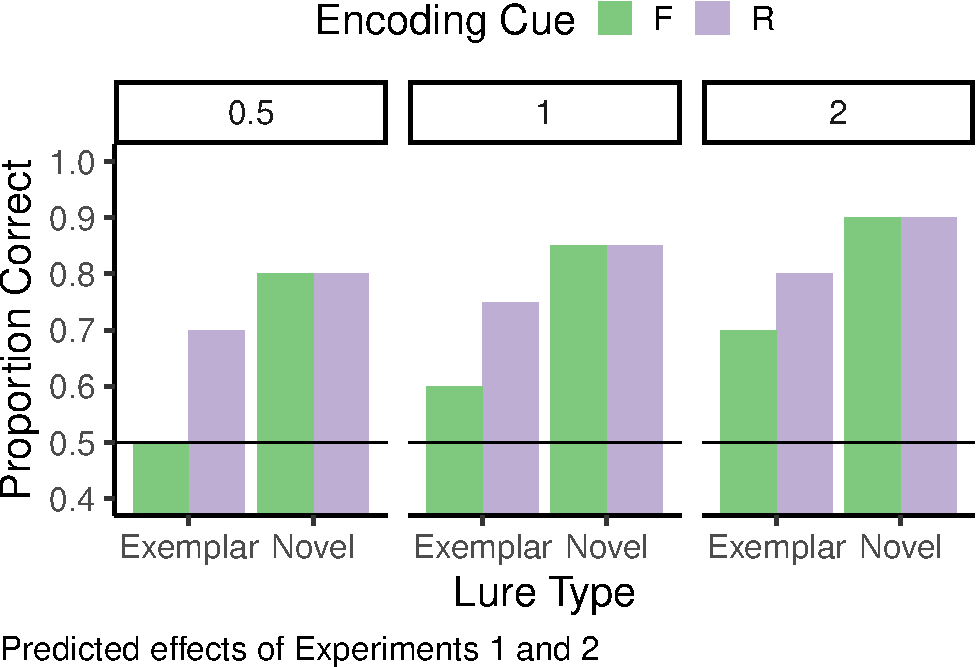
\includegraphics[width=1\linewidth]{Ihejirika_honors_thesis_Spring_2022_files/figure-latex/power-1} \caption{Predicted effects of the stimulus duration manipulation on the size directed forgetting for exemplar and novel test items.}\label{fig:power}
\end{figure}

\hypertarget{experiment-1}{%
\section{Experiment 1}\label{experiment-1}}

Experiment 1 quite similarly resembles the traditional directed forgetting procedural technique used by Bjork, Laberge, and Legrand (1968) to explore participant recognition of previously seen encoding stimuli when randomly presented with distractors throughout the testing phase. Deviations from Bjork's experimental procedure include (1) the factorial manipulation of stimuli presentation duration by 500 milliseconds, 1 second and 2 seconds (2) the randomized presentation of novel and exemplar distractors throughout the testing phase (3) the use of inherently more memorable stimuli -images- throughout both the encoding and testing phase, instead of word stimuli.

\hypertarget{method}{%
\subsection{Method}\label{method}}

\hypertarget{participants}{%
\subsubsection{Participants}\label{participants}}

A total of 47 participants were recruited from Amazon's Mechanical Turk (Crump, McDonnell, \& Gureckis, 2013). Mean age was 34.90 (range = 22 to 60). There were 23 females, and 24 males. There were 41 right-handed participants, and NA left or both handed participants. 37 participants reported normal vision, and 10 participants reported corrected-to-normal vision. 37 participants reported English as a first language, and 10 participants reported English as a second language.

\hypertarget{stimuli-and-apparatus.}{%
\subsubsection{Stimuli and Apparatus.}\label{stimuli-and-apparatus.}}

There were 120 images from a total of 16 categorical scenes presented throughout the encoding phase of this experiment. These sixteen categorical scenes were further classified as being either outdoor scenes or indoor scenes. The eight of sixteen outdoor visual scenes consisted of settings which included bedrooms, churches, classrooms, offices, dining rooms, conference rooms, hair salons \& empty rooms. The eight of sixteen indoor visual scenes consisted of settings such as airports, bridges, beaches, castles, cemeteries, houses, tents and playgrounds. These 120 images were of the same database of 320 total images of 24 different categorical scenes created by Brady et al. (2008). This was the same image set used by Ahmad et al. (2019).

Alongside the initial 120 images presented during the encoding phase, another 120 images were selected as distractors throughout the testing phase. Sixty of these images were of the same visual scene categories as the images presented during the encoding phase. These images were presented as exemplar distractor testing conditions. The other half of the 120 distractor images were of completely new visual scene categories as the images presented throughout the encoding phase. These distractor images were presented as novel distractor testing conditions. This experiment was programmed in JavaScript using Jspsych and was served onto the web using Jatos. The results of this experiment were analyzed using R code.

We used R (Version 4.1.0; R Core Team, 2021) and the R-packages \emph{data.table} (Version 1.14.2; Dowle \& Srinivasan, 2021), \emph{dplyr} (Version 1.0.8; Wickham, François, Henry, \& Müller, 2021), \emph{fontawesome} (Version 0.2.2; Iannone, 2021), \emph{forcats} (Version 0.5.1; Wickham, 2021a), \emph{ggplot2} (Version 3.3.5; Wickham, 2016), \emph{jsonlite} (Version 1.8.0; Ooms, 2014), \emph{pacman} (Version 0.5.1; Rinker \& Kurkiewicz, 2018), \emph{papaja} (Version 0.1.0.9997; Aust \& Barth, 2020), \emph{purrr} (Version 0.3.4; Henry \& Wickham, 2020), \emph{readr} (Version 2.1.2; Wickham \& Hester, 2021), \emph{stringr} (Version 1.4.0; Wickham, 2019), \emph{tibble} (Version 3.1.6; Müller \& Wickham, 2021), \emph{tidyr} (Version 1.2.0; Wickham, 2021b), \emph{tidyverse} (Version 1.3.1; Wickham et al., 2019), \emph{tinylabels} (Version 0.2.3; Barth, 2021), and \emph{xtable} (Version 1.8.4; Dahl, Scott, Roosen, Magnusson, \& Swinton, 2019) for all our analyses. We collected five subjects worth of pilot data. For each subject we computed mean recognition accuracy in each condition of the design. Figure 1 shows mean recognition accuracy in each condition, collapsed across each subject.

\hypertarget{design}{%
\subsubsection{Design}\label{design}}

This experiment consisted of a 2x2x3 completely within-subjects experimental design, with the manipulated variables including the Distractor Test, Cue \& picture encoding time. The distractor testing condition variable possessed two distinct manipulations, being novel testing conditions and exemplar testing conditions. Novel testing conditions display images with previously unseen or unrelated visual scene categories as distractors during the testing phase. Exemplar testing conditions display images with similar visual scene categories as distractors during the testing phase. The picture presentation time variable possessed three distinct manipulations to the duration of images presented during the encoding phase of the experiment. These three manipulations included durations of 500 milliseconds, 1 second and 2 seconds. The cue presentation variable possessed two distinct manipulations. These two manipulations included the ``Remember'' cue and the ``Forget'' cue. The Remember cue instructs participants to remember the upcoming image stimuli, while the ``Forget'' cue instructs participants to selectively forget the upcoming image stimuli.

\hypertarget{procedure}{%
\subsection{Procedure}\label{procedure}}

We used the Just Another Tool for Online Studies (JATOS) to serve the website containing the experiment (Lange, Kühn, \& Filevich, 2015). The experiment was programmed using JsPsych (De Leeuw, 2015). The source code for the experiments is available from the project website (see author note).

As stated earlier, there were two major phases of the experiment. These phases are the encoding phase and the testing phase. Prior to the encoding phase however, participants were presented with a consent form. Upon completion of the consent form, they were presented with encoding phase instructions.

During the encoding phase, participants were presented with 120 trials. On each trial an image was presented followed by an instructional cue to remember (R) or forget (F) the image. The image was presented for 500 ms, 1000ms, or 2000 ms. Stimulus duration was randomized across trials. The instructional cue was always presented for 2000 ms. Half of the trials involved a remember cue, and the other half involved a forget cue. The instructional cue was randomized across trials. The image stimuli were selected randomly from 10 image categories. Each participant received a differenet subset of random images.

Upon completion of the encoding phase, participants were then taken to the testing phase. Similarly to the encoding phase, during the beginning of the testing phase participants were given instructions of completing the testing phase. During the testing phase, participants are given a series of trials where they were shown either an exemplar distractor image or a novel distractor image alongside an image previously seen during the encoding phase and are tasked with selecting the encoding image. There were 60 novel distractor images and 60 exemplar distractor images, each of which were presented at random throughout the testing procedure. Novel distractors were images from categories not presented at encoding. Exemplar distractors were images from the same category as presented during encoding.

\hypertarget{data-exclusion}{%
\subsection{Data-Exclusion}\label{data-exclusion}}

Our participants were recruited online and completed the experiment from a web browser. Our experiment script requests that participants attempt the task to the best of their ability. Nevertheless, it is possible that participants complete the experiment and submit data without attempting to complete the task as directed. We developed a set of criteria to exclude participants whose performance indicated they were not attempting the task as instructed. These criteria also allowed us to confirm that the participants we included in the analysis did attempt the task as instructed to the best of their ability. We adopted the following five criteria:

First, during the encoding phase participants responded to each instructional cue (to remember or forget the picture on each trial) by pressing ``R'' or ``F'' on the keyboard. This task demand further served as an attentional check. We excluded participants who scored lower than 75\% correct on instructional cue identification responses. Second, participants who did not respond on more than 25\% of trials in the recognition test were excluded. Third, we measured response bias (choosing the left or right picture) during the recognition test, and excluded participants who made 75\% of their responses to one side (indicating they were repeatedly pressing the same button on each trial). Fourth, we excluded participants whose mean reaction time during the recognition test was less than 300ms, indicating they were pressing the buttons as fast as possible without making a recognition decision. Finally, we computed mean accuracy for the novel lure condition for all participants, and excluded participants whose mean accuracy was less than 55\% for those items. All together 13 participants were excluded.

\hypertarget{results}{%
\subsection{Results}\label{results}}

\begin{figure}
\centering
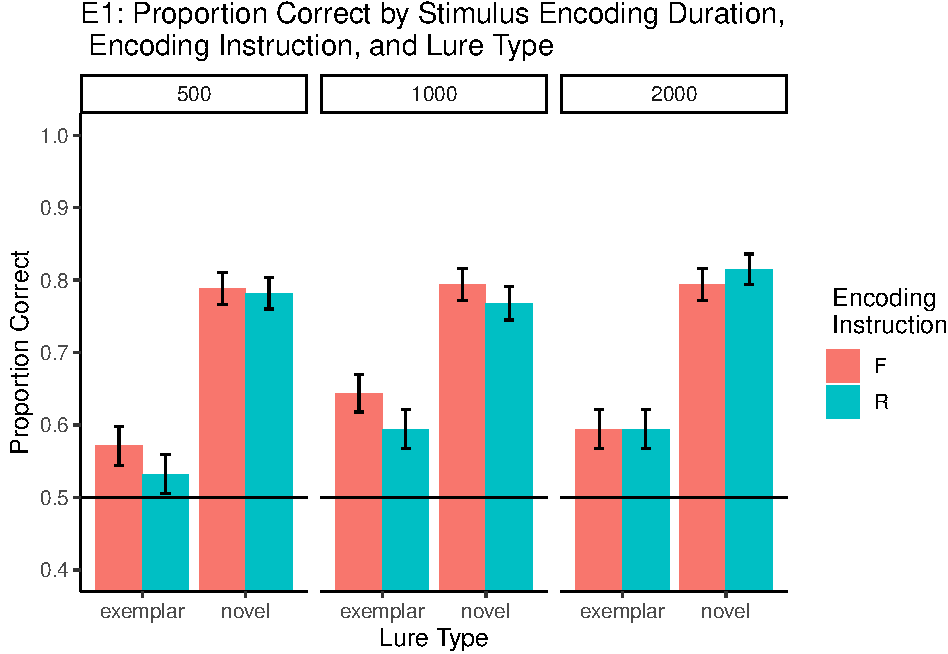
\includegraphics{Ihejirika_honors_thesis_Spring_2022_files/figure-latex/e1fig-1.pdf}
\caption{\label{fig:e1fig}Mean proportion correct as a function of encoding duration, encoding cue, and lure type for Experiment 1.}
\end{figure}

\hypertarget{proportion-correct}{%
\subsubsection{Proportion Correct}\label{proportion-correct}}

The proportion of accurately recognized encoding stimuli was collected for each of the subjects who participated in the pilot study. The recorded proportions were then averaged according to the conditions present in this 2x2x3 within subjects experimental design. Mean proportion correct for each subject was then submitted to a 2: Cue instruction conditions (R vs F), by 2: Test conditions (Novel vs Exemplar), by 3: Stimulus duration conditions (500ms vs 1000ms vs 2000ms), repeated measures analysis of variance.

Proportion correct for each subject in each condition was submitted to a 3 (Encoding Duration: 500ms, 1000ms, 2000ms) x 2 (Encoding Instruction: Forget vs.~Remember) x 2 (Lure type: Novel vs.~Exemplar) fully repeated measures ANOVA. For completeness, each main effect and higher-order interaction is described in turn.

The main effect of encoding duration was not significant, \(F(2, 66) = 2.62\), \(p = .080\), \(\hat{\eta}^2_G = .007\), 90\% CI \([.000, .048]\). Proportion correct was similar across the 500 ms (M = 0.668, SEM = 0.013), 1000 ms (M = 0.7, SEM = 0.012), and 2000 ms (M = 0.699, SEM = 0.012) stimulus durations.

The main effect of encoding instruction was not significant, \(F(1, 33) = 1.95\), \(p = .171\), \(\hat{\eta}^2_G = .002\), 90\% CI \([.000, .005]\). Proportion correct was similar for remember cues (M = 0.681, SEM = 0.01) and forget cues (M = 0.698, SEM = 0.01).

The main effect of lure type was significant, \(F(1, 33) = 133.34\), \(p < .001\), \(\hat{\eta}^2_G = .257\), 90\% CI \([.070, .444]\). Proportion correct was higher for novel lures (M = 0.79, SEM = 0.009) than exemplar lures (M = 0.588, SEM = 0.011).

The main question of interest was whether directing forgetting would vary across the encoding duration times. The interaction between encoding instruction and encoding duration was, \(F(2, 66) = 0.95\), \(p = .393\), \(\hat{\eta}^2_G = .003\), 90\% CI \([.000, .024]\).

Paired sample t-tests were used to assess the directed forgetting effect at each encoding duration. The directed forgetting effect is taken as the difference between proportion correct for remember minus forget items. At 500 ms, the directed forgetting effect was reversed and not significant, \(M = -0.02\), 95\% CI \([-0.07, 0.03]\), \(t(33) = -0.86\), \(p = .398\). At 1000ms, the directed forgetting effect was reversed and not significant, \(M = -0.04\), 95\% CI \([-0.09, 0.01]\), \(t(33) = -1.61\), \(p = .118\). And, at 2000 ms, the directed forgetting effect was again not detected, \(M = 0.01\), 95\% CI \([-0.03, 0.06]\), \(t(33) = 0.47\), \(p = .643\).

The encoding duration by lure type interaction was, \(F(2, 66) = 2.99\), \(p = .057\), \(\hat{\eta}^2_G = .008\), 90\% CI \([.000, .049]\). In the 500 ms condition, proportion correct was higher for novel than exemplar lures, \(M = 0.23\), 95\% CI \([0.19, 0.28]\), \(t(33) = 10.00\), \(p < .001\). The advantage for novel over exemplar items was smaller in the 1000 ms condition, \(M = 0.16\), 95\% CI \([0.11, 0.21]\), \(t(33) = 6.80\), \(p < .001\), and 2000 ms condition \(M = 0.21\), 95\% CI \([0.16, 0.26]\), \(t(33) = 7.91\), \(p < .001\).

The encoding instruction by lure type interaction was not significant, \(F(1, 33) = 1.24\), \(p = .273\), \(\hat{\eta}^2_G = .001\), 90\% CI \([.000, .069]\). Similarly, the interaction between encoding duration, instruction, and lure type was not significant, \(F(2, 66) = 0.01\), \(p = .988\), \(\hat{\eta}^2_G = .000\), 90\% CI \([.000, .000]\).

\hypertarget{reaction-times}{%
\subsubsection{Reaction times}\label{reaction-times}}

\begin{figure}
\centering
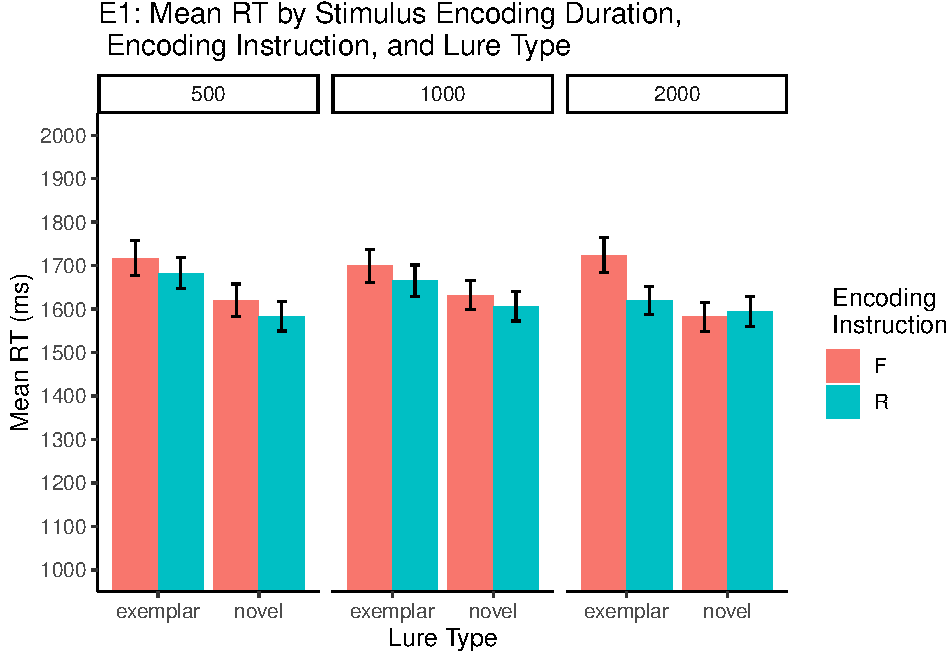
\includegraphics{Ihejirika_honors_thesis_Spring_2022_files/figure-latex/E1fig2-1.pdf}
\caption{\label{fig:E1fig2}Mean reaction times as a function of encoding duration, encoding instruction, and test lure type for Experiment 1.}
\end{figure}

Mean reaction times on correct trials for each subject in each condition were submitted to a 3 (Encoding Duration: 500ms, 1000ms, 2000ms) x 2 (Encoding Instruction: Forget vs.~Remember) x 2 (Lure type: Novel vs.~Exemplar) fully repeated measures ANOVA. For brevity we report only the significant effects. The full analysis is contained in supplementary materials.

The main effect of encoding instruction was significant, \(F(1, 33) = 5.44\), \(p = .026\), \(\hat{\eta}^2_G = .003\), 90\% CI \([.000, .092]\). Mean reaction times were faster for choosing remember cued items (M = 1625.191, SEM = 13.987) than forget cued items (M = 1662.582, SEM = 15.328).

The main effect of lure type was significant, \(F(1, 33) = 6.74\), \(p = .014\), \(\hat{\eta}^2_G = .011\), 90\% CI \([.000, .130]\). Mean reaction times were faster in the novel lure condition (M = 1603.181, SEM = 14.07) than exemplar lure condition (M = 1684.996, SEM = 15.225).

The remaining main effects and interactions were not significant.

\hypertarget{discussion}{%
\subsection{Discussion}\label{discussion}}

Resulting analysis of data gathered fails to identify several main effects between the experimental conditions of Stimuli Duration and Encoding Instruction on the mean proportion of correctly recognized visual scenes, yet identifies a main effect of lure condition.
There also appears to be a strong interaction effect between encoding duration and lure condition.

Results of experiment 1 fails to replicate the findings of Ahmad et al. (2019) at 2000ms, and also fails to support the initial prediction of increased effect magnitudes for exemplar conditions from 2000ms to 1000ms to finally 500ms. Several reversed directed forgetting effects were observed for exemplar lures at 1000ms and 500ms conditions. Potential explanations of the reversed directed forgetting effect observed in Experiment 1 were explored.

These explanations included experimental programming errors and noise yielded from the random encoding image durations. Potential programming errors includes the mislabeling of remember-cued and forget-cued encoding instructions for the 1000ms encoding duration condition. After closely reviewing the code however, this explanation is shown to be incorrect.

According to the previous research exploring the effects of surprise on memory, noise yielded from the random presentation of images at 2000ms, 1000ms and 500ms durations would make more difficult for participants to reliably process the encoding cues. This explanation is explored in experiment 2, as I present identical visual scenes in blocks of 500ms, 1000ms and 2000ms. The incorporation of a blocked procedure will allow me to further replicate experimental conditions of Ahmad et al. (2019), to observe whether we will receive similar results.

Additional data of reaction time was also recorded and analyzed. Significant main effects of encoding instuctions and lure conditions were the only observed main effects.

\hypertarget{experiment-2}{%
\section{Experiment 2}\label{experiment-2}}

A potential explanation of experiment 1's failure to replicate Ahmad et al. (2019) is the randomized manipulations to stimulus presentation duration from 500ms, 1000ms and 2000ms. In experiment 1 participants may have had difficulty intentionally forgetting because of the stimulus duration changed randomly on each trial.

Experiment 2 resolves this using blocked stimulus duration conditions with three total blocks. Stimulus encoding duration consists of 500ms, 1000ms and 2000ms for 1/3 of block conditions each. These blocks are randomized across participants. However, within a block of trials, participants receive a consistant stimulus duration on each trial.

Block designs allow a closer replication of both Ahmad Tan \& Hockley and Experiment 1 (i.e., the 2000 ms condition). By doing this, one can determine whether effects detailed by Ahmad Tan and Hockley, and experiment 1 are observed only in conditions specific to each experiment, thus reducing the generalizability of their results.

A directed forgetting effect intensity similar to that observed by Ahmad et al.~is expected for 2000ms blocked conditions, as it is an identical replication of their methodology. Similarly, we expect to find progressive lower DFE magnitudes from 2000ms blocks to 1000ms blocks to 500ms blocks. Finally, we expect to observe higher DFE magnitudes for novel test conditions than exemplar test conditions, as novel conditions require the recognition of the lowest gistidual details.

\hypertarget{method-1}{%
\subsection{Method}\label{method-1}}

\hypertarget{participants-1}{%
\subsubsection{Participants}\label{participants-1}}

A total of 45 participants were recruited from Amazon's Mechanical Turk. Mean age was 37.90 (range = 25 to 65 ). There were 11 females, and 34 males. There were 42 right-handed participants, and NA left or both handed participants. 36 participants reported normal vision, and 8 participants reported corrected-to-normal vision. 41 participants reported English as a first language, and 4 participants reported English as a second language.

\hypertarget{stimuli-and-apparatus}{%
\subsubsection{Stimuli and Apparatus}\label{stimuli-and-apparatus}}

The stimuli and apparatus were the same as Experiment 1.

\hypertarget{design-1}{%
\subsubsection{Design}\label{design-1}}

This experiment consisted of a 2x2x3 completely within-subjects experimental design, with the manipulated variables including the Distractor Test, Cue Instruction \& Picture encoding time. The distractor testing condition variable possessed two distinct manipulations, being novel testing conditions and exemplar testing conditions. Novel testing conditions display images with previously unseen or unrelated visual scene categories as distractors during the testing phase. Exemplar testing conditions display images with similar visual scene categories as distractors during the testing phase. The picture presentation time variable possessed three distinct manipulations to the duration of images presented during the encoding phase of the experiment. These three manipulations included durations of 500 milliseconds, 1 second and 2 seconds. The cue presentation variable possessed two distinct manipulations. These two manipulations included the ``Remember'' cue and the ``Forget'' cue. The Remember cue instructs participants to remember the upcoming image stimuli, while the ``Forget'' cue instructs participants to selectively forget the upcoming image stimuli.

\hypertarget{procedure-1}{%
\subsection{Procedure}\label{procedure-1}}

The procedure for Experiment 2 was the same as Experiment 1, except for the presentation of image stimuli in blocks of 500ms, 1000ms and 2000ms. As stated earlier, there were two major phases of the experiment. These phases are the encoding phase and the testing phase. Prior to the encoding phase however, participants were presented with a consent form. Upon completion of the consent form, they were presented with encoding phase instructions.

\hypertarget{data-exclusions}{%
\subsection{Data-exclusions}\label{data-exclusions}}

We used the same exclusion criteria as set of Experiment 1. 6 participants were excluded from the analysis in Experiment 2.

\hypertarget{results-1}{%
\subsection{Results}\label{results-1}}

\begin{figure}
\centering
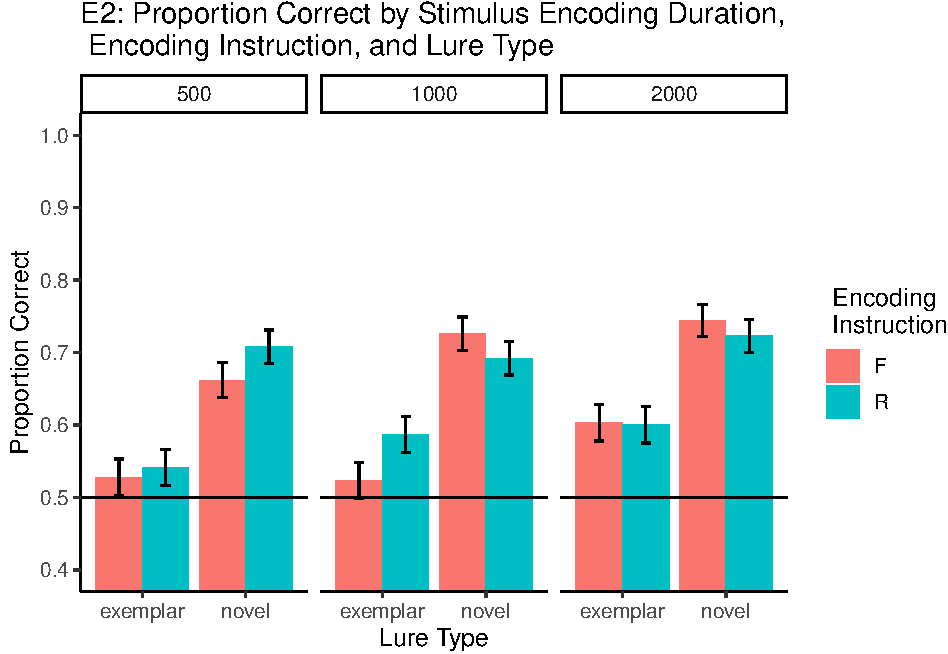
\includegraphics{Ihejirika_honors_thesis_Spring_2022_files/figure-latex/e2fig1-1.pdf}
\caption{\label{fig:e2fig1}Mean proportion correct as a function of encoding duration, encoding cue, and lure type for Experiment 2.}
\end{figure}

\hypertarget{proportion-correct-1}{%
\subsubsection{Proportion Correct}\label{proportion-correct-1}}

Proportion correct for each subject in each condition was submitted to a 3 (Encoding Duration: 500ms, 1000ms, 2000ms) x 2 (Encoding Instruction: Forget vs.~Remember) x 2 (Lure type: Novel vs.~Exemplar) fully repeated measures ANOVA. For completeness, each main effect and higher-order interaction is described in turn.

The main effect of encoding duration was significant, \(F(2, 76) = 5.54\), \(p = .006\), \(\hat{\eta}^2_G = .017\), 90\% CI \([.000, .074]\). Proportion correct was lowest for the 500 ms duration (M = 0.61, SEM = 0.012), and higher for the 1000 ms (M = 0.632, SEM = 0.012), and 2000 ms (M = 0.667, SEM = 0.012) stimulus durations.

The main effect of encoding instruction was not significant, \(F(1, 38) = 0.65\), \(p = .425\), \(\hat{\eta}^2_G = .001\), 90\% CI \([.000, .055]\). Proportion correct was similar for remember cues (M = 0.642, SEM = 0.01) and forget cues (M = 0.631, SEM = 0.01).

The main effect of lure type was significant, \(F(1, 38) = 79.66\), \(p < .001\), \(\hat{\eta}^2_G = .137\), 90\% CI \([.014, .312]\). Proportion correct was higher for novel lures (M = 0.709, SEM = 0.009) than exemplar lures (M = 0.564, SEM = 0.01).

The main question of interest was whether directing forgetting would vary across the encoding duration times. The interaction between encoding instruction and encoding duration was not significant, \(F(2, 76) = 0.83\), \(p = .441\), \(\hat{\eta}^2_G = .002\), 90\% CI \([.000, .013]\).

Paired sample t-tests were used to assess the directed forgetting effect at each encoding duration. The directed forgetting effect is taken as the difference between proportion correct for remember minus forget items. At 500 ms, the directed forgetting effect was not significant, \(M = 0.03\), 95\% CI \([-0.01, 0.07]\), \(t(38) = 1.36\), \(p = .181\). At 1000ms, the directed forgetting effect was not significant, \(M = 0.02\), 95\% CI \([-0.03, 0.06]\), \(t(38) = 0.63\), \(p = .531\). And, at 2000 ms, the directed forgetting effect was again not detected, \(M = -0.01\), 95\% CI \([-0.06, 0.04]\), \(t(38) = -0.49\), \(p = .629\).

The encoding duration by lure type interaction was not significnat, \(F(2, 76) = 0.26\), \(p = .775\), \(\hat{\eta}^2_G = .001\), 90\% CI \([.000, .000]\). The encoding instruction by lure type interaction was not significant, \(F(1, 38) = 1.13\), \(p = .295\), \(\hat{\eta}^2_G = .001\), 90\% CI \([.000, .065]\). Similarly, the interaction between encoding duration, instruction, and lure type was not significant, \(F(2, 76) = 2.42\), \(p = .095\), \(\hat{\eta}^2_G = .005\), 90\% CI \([.000, .037]\).

\hypertarget{reaction-times-1}{%
\subsubsection{Reaction times}\label{reaction-times-1}}

\begin{figure}
\centering
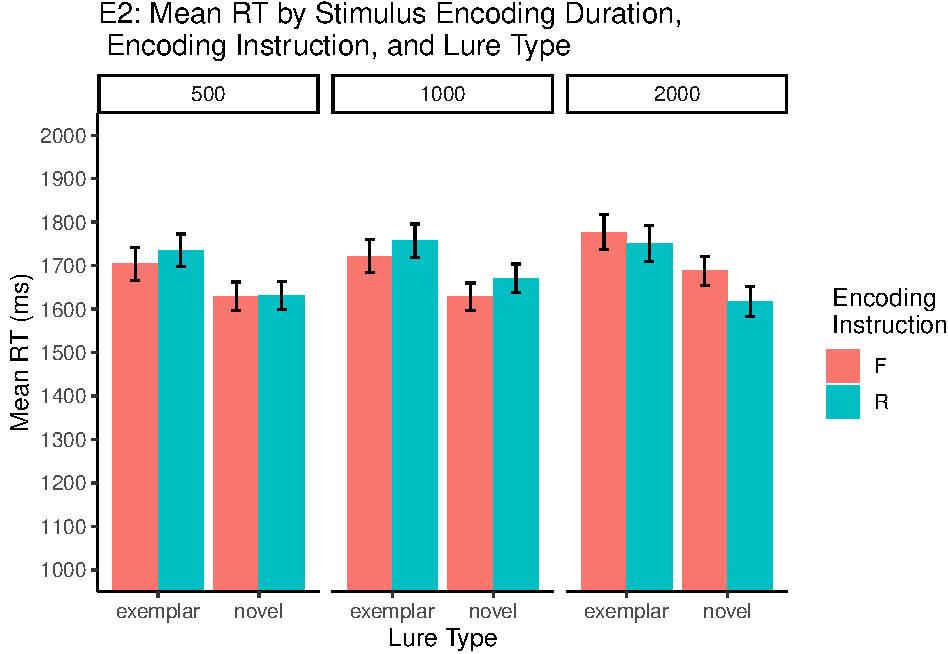
\includegraphics{Ihejirika_honors_thesis_Spring_2022_files/figure-latex/E2fig2-1.pdf}
\caption{\label{fig:E2fig2}Mean reaction times as a function of encoding duration, encoding instruction, and test lure type for Experiment 2.}
\end{figure}

Mean reaction times on correct trials for each subject in each condition were submitted to a 3 (Encoding Duration: 500ms, 1000ms, 2000ms) x 2 (Encoding Instruction: Forget vs.~Remember) x 2 (Lure type: Novel vs.~Exemplar) fully repeated measures ANOVA. For brevity we report only the significant effects. The full analysis is contained in supplementary materials.

The main effect of lure type was significant, \(F(1, 38) = 7.32\), \(p = .010\), \(\hat{\eta}^2_G = .014\), 90\% CI \([.000, .128]\). Mean reaction times were faster in the novel lure condition (M = 1644.224, SEM = 13.401) than exemplar lure condition (M = 1741.122, SEM = 15.939).

The remaining main effects and interactions were not significant.

\hypertarget{discussion-1}{%
\subsection{Discussion}\label{discussion-1}}

The results of Experiment 2 again did not show clear evidence of a directed forgetting effect for natural scenes. As with Experiment 1, in the 2000 ms stimulus duration condition, we were unable to replicate the directed forgetting effect reported by @Ahmad et al. (2019).

\hypertarget{general-discussion}{%
\section{General Discussion}\label{general-discussion}}

Overall, we failed to replicate the findings of Ahmad et al. (2019) across both experiments for 2000ms. We also failed to obtain experimental results which support initial predictions of an increased directed forgetting effect magnitude for exemplar conditions from 2000ms to 1000ms to 500ms. A potential explanation of this lies in the number of participants ran across both experiments. Initial power analyses estimated that nearly 200 participants would be required for the predicted results to occur, yet only 47 and 45 participants were ran in experiments 1 and 2 respectively. Higher proportions of correctly recognized images were observed during experiment 1 for Forget-cues than Remember-cues for exemplar conditions at 500ms and 1000ms, and novel lure conditions at 1000ms. Directed forgetting effects could be observed during experiment 2 for novel conditions at 500ms and for exemplar conditions at 1000ms conditions, while a reversed directed forgetting effect can be observed for novel conditions at 1000ms and 2000ms conditions.

There are several experimental limitations which serve to explain our failure to provide evidence of a Trace Strength Account and replicate the findings of Ahmad et al. (2019). One such limitation is the number of participants across both experiment 1 and experiment 2. A priori power analysis indicated that at least 200 subjects would be required for the detection of the predicted three-way interaction between the directed forgetting effect, stimulus duration, and test conditions. Results of the 45 participants ran in Experiment 2 and 47 ran in Experiment 1 may be noisy.

Future research could improve this failure to observe a large effect of the stimulus duration manipulation by considering manipulations that should influence image encoding strength. These could include, 1) making duration even shorter or even longer; 2) adding more images; 3) making the images less distinctive by showing more images from the same category; and, 4) presenting images with various levels of distortion. All of these encoding manipulations could provide further tests of the memory strength hypothesis.

Additionally, further cue manipulations should be considered to make the cues even more effective and increase the magnitude intentional forgetting. Such manipulations include, 1) reduction in the number of trials; 2) incorporation of the list method instead of the item method; 3) presentation of subjects with quizzes on the instructions to make sure they understand them; and, 4) randomly presenting subjects with attention checks to ask people how much they are trying, and/or how much they feel they are being successful. These manipulations may provide solutions to current experimental issues of 1) subjects failing to understand task instructions; 2) failure to check if people are actively carrying out the instructions on a trial-to-trial basis; 3) participants fatiguing throughout the experiment, leading to boredom and reductions in effort; and, 4) motivated subjects who are trying on each trial, finding it difficult to comply with instructions successfully because the timing of cue presentation is fairly rapid.

\hypertarget{conclusion}{%
\section{Conclusion}\label{conclusion}}

The ability to selectively remember or selectively forget information is important, as people sometimes want to remember and sometimes want to forget events or experiences. With this being said, memorable memories can be especially hard to forget. We tested whether memorable stimuli such as pictures could be intentionally forgotten. In particular, we were interested in whether making pictures less memorable by reducing encoding duration would allow people more control over whether they wanted to remember or forget each picture. We found limited evidence of directed forgetting effects and considered ways to improve future experiments in this area.

\newpage

\hypertarget{references}{%
\section{References}\label{references}}

\begingroup
\setlength{\parindent}{-0.5in}
\setlength{\leftskip}{0.5in}

\hypertarget{refs}{}
\begin{CSLReferences}{1}{0}
\leavevmode\vadjust pre{\hypertarget{ref-ahmadEffectsVaryingPresentation2017}{}}%
Ahmad, F. N., Moscovitch, M., \& Hockley, W. E. (2017). Effects of varying presentation time on long-term recognition memory for scenes: {Verbatim} and gist representations. \emph{Memory \& Cognition}, \emph{45}(3), 390--403. \url{https://doi.org/gmgg4q}

\leavevmode\vadjust pre{\hypertarget{ref-ahmadDirectedForgettingCategorised2019}{}}%
Ahmad, F. N., Tan, P., \& Hockley, W. E. (2019). Directed forgetting for categorised pictures: Recognition memory for perceptual details versus gist. \emph{Memory}, \emph{27}(7), 894--903. \url{https://doi.org/gmgg3g}

\leavevmode\vadjust pre{\hypertarget{ref-R-papaja}{}}%
Aust, F., \& Barth, M. (2020). \emph{{papaja}: {Prepare} reproducible {APA} journal articles with {R Markdown}}. Retrieved from \url{https://github.com/crsh/papaja}

\leavevmode\vadjust pre{\hypertarget{ref-R-tinylabels}{}}%
Barth, M. (2021). \emph{{tinylabels}: Lightweight variable labels}. Retrieved from \url{https://github.com/mariusbarth/tinylabels}

\leavevmode\vadjust pre{\hypertarget{ref-bjorkTheoreticalImplicationsDirected1972}{}}%
Bjork, R. A. (1972). Theoretical implications of directed forgetting. In A. W. Melton \& E. Martin (Eds.), \emph{Coding processes in human memory} (pp. 217--235). {Washington, DC}: {Winston}.

\leavevmode\vadjust pre{\hypertarget{ref-bjorkModificationShorttermMemory1968}{}}%
Bjork, R. A., Laberge, D., \& Legrand, R. (1968). The modification of short-term memory through instructions to forget. \emph{Psychonomic Science}, \emph{10}(2), 55--56. \url{https://doi.org/gmt488}

\leavevmode\vadjust pre{\hypertarget{ref-bradyVisualLongtermMemory2008}{}}%
Brady, T. F., Konkle, T., Alvarez, G. A., \& Oliva, A. (2008). Visual long-term memory has a massive storage capacity for object details. \emph{Proceedings of the National Academy of Sciences}, \emph{105}(38), 14325--14329. \url{https://doi.org/c268jz}

\leavevmode\vadjust pre{\hypertarget{ref-crump2013evaluating}{}}%
Crump, M. J., McDonnell, J. V., \& Gureckis, T. M. (2013). Evaluating amazon's mechanical turk as a tool for experimental behavioral research. \emph{PloS One}, \emph{8}(3), e57410.

\leavevmode\vadjust pre{\hypertarget{ref-R-xtable}{}}%
Dahl, D. B., Scott, D., Roosen, C., Magnusson, A., \& Swinton, J. (2019). \emph{Xtable: Export tables to LaTeX or HTML}. Retrieved from \url{https://CRAN.R-project.org/package=xtable}

\leavevmode\vadjust pre{\hypertarget{ref-de2015jspsych}{}}%
De Leeuw, J. R. (2015). jsPsych: A JavaScript library for creating behavioral experiments in a web browser. \emph{Behavior Research Methods}, \emph{47}(1), 1--12.

\leavevmode\vadjust pre{\hypertarget{ref-R-data.table}{}}%
Dowle, M., \& Srinivasan, A. (2021). \emph{Data.table: Extension of `data.frame`}. Retrieved from \url{https://CRAN.R-project.org/package=data.table}

\leavevmode\vadjust pre{\hypertarget{ref-EpsteinW1972}{}}%
Epstein, D. W. W., William. Massaro. (1972). Selective search in directed forgetting. \emph{Journal of Experimental Psychology}, \emph{94}(1), 18--24. \url{https://doi.org/10.1037/h0032791}

\leavevmode\vadjust pre{\hypertarget{ref-R-purrr}{}}%
Henry, L., \& Wickham, H. (2020). \emph{Purrr: Functional programming tools}. Retrieved from \url{https://CRAN.R-project.org/package=purrr}

\leavevmode\vadjust pre{\hypertarget{ref-hintzmanSchemaAbstractionMultipleTrace1986}{}}%
Hintzman, D. L. (1986). "{Schema Abstraction}" in a {Multiple-Trace Memory Model}. \emph{Psychological Review}, \emph{93}, 411--428. \url{https://doi.org/bzdsr4}

\leavevmode\vadjust pre{\hypertarget{ref-R-fontawesome}{}}%
Iannone, R. (2021). \emph{Fontawesome: Easily work with 'font awesome' icons}. Retrieved from \url{https://CRAN.R-project.org/package=fontawesome}

\leavevmode\vadjust pre{\hypertarget{ref-lange2015just}{}}%
Lange, K., Kühn, S., \& Filevich, E. (2015). Just another tool for online studies (JATOS): An easy solution for setup and management of web servers supporting online studies. \emph{PloS One}, \emph{10}(6), e0130834.

\leavevmode\vadjust pre{\hypertarget{ref-macleodDirectedForgetting1998}{}}%
MacLeod, C. M. (1998). Directed forgetting. In J. M. Golding \& C. M. MacLeod (Eds.), \emph{Intentional forgetting: {Interdisciplinary} approaches} (pp. 1--57). {Mahwah, NJ}: {Lawrence Erlbaum Associates}.

\leavevmode\vadjust pre{\hypertarget{ref-R-tibble}{}}%
Müller, K., \& Wickham, H. (2021). \emph{Tibble: Simple data frames}. Retrieved from \url{https://CRAN.R-project.org/package=tibble}

\leavevmode\vadjust pre{\hypertarget{ref-R-jsonlite}{}}%
Ooms, J. (2014). The jsonlite package: A practical and consistent mapping between JSON data and r objects. \emph{arXiv:1403.2805 {[}Stat.CO{]}}. Retrieved from \url{https://arxiv.org/abs/1403.2805}

\leavevmode\vadjust pre{\hypertarget{ref-R-base}{}}%
R Core Team. (2021). \emph{R: A language and environment for statistical computing}. Vienna, Austria: R Foundation for Statistical Computing. Retrieved from \url{https://www.R-project.org/}

\leavevmode\vadjust pre{\hypertarget{ref-R-pacman}{}}%
Rinker, T. W., \& Kurkiewicz, D. (2018). \emph{{pacman}: {P}ackage management for {R}}. Buffalo, New York. Retrieved from \url{http://github.com/trinker/pacman}

\leavevmode\vadjust pre{\hypertarget{ref-standingLearning10000Pictures1973}{}}%
Standing, L. (1973). Learning 10000 pictures. \emph{The Quarterly Journal of Experimental Psychology}, \emph{25}(2), 207--222. \url{https://doi.org/fnjhs5}

\leavevmode\vadjust pre{\hypertarget{ref-weiner1969effects}{}}%
Weiner, B., \& Reed, H. (1969). Effects of the instructional sets to remember and to forget on short-term retention: Studies of rehearsal control and retrieval inhibition (repression). \emph{Journal of Experimental Psychology}, \emph{79}(2p1), 226.

\leavevmode\vadjust pre{\hypertarget{ref-WetzelC1977}{}}%
Wetzel, R. E., Douglas C. Hunt. (1977). Cue delay and the role of rehearsal in directed forgetting. \emph{Journal of Experimental Psychology: Human Learning and Memory}, \emph{3}(2), 233--245. \url{https://doi.org/10.1037/0278-7393.3.2.233}

\leavevmode\vadjust pre{\hypertarget{ref-R-ggplot2}{}}%
Wickham, H. (2016). \emph{ggplot2: Elegant graphics for data analysis}. Springer-Verlag New York. Retrieved from \url{https://ggplot2.tidyverse.org}

\leavevmode\vadjust pre{\hypertarget{ref-R-stringr}{}}%
Wickham, H. (2019). \emph{Stringr: Simple, consistent wrappers for common string operations}. Retrieved from \url{https://CRAN.R-project.org/package=stringr}

\leavevmode\vadjust pre{\hypertarget{ref-R-forcats}{}}%
Wickham, H. (2021a). \emph{Forcats: Tools for working with categorical variables (factors)}. Retrieved from \url{https://CRAN.R-project.org/package=forcats}

\leavevmode\vadjust pre{\hypertarget{ref-R-tidyr}{}}%
Wickham, H. (2021b). \emph{Tidyr: Tidy messy data}. Retrieved from \url{https://CRAN.R-project.org/package=tidyr}

\leavevmode\vadjust pre{\hypertarget{ref-R-tidyverse}{}}%
Wickham, H., Averick, M., Bryan, J., Chang, W., McGowan, L. D., François, R., \ldots{} Yutani, H. (2019). Welcome to the {tidyverse}. \emph{Journal of Open Source Software}, \emph{4}(43), 1686. \url{https://doi.org/10.21105/joss.01686}

\leavevmode\vadjust pre{\hypertarget{ref-R-dplyr}{}}%
Wickham, H., François, R., Henry, L., \& Müller, K. (2021). \emph{Dplyr: A grammar of data manipulation}. Retrieved from \url{https://CRAN.R-project.org/package=dplyr}

\leavevmode\vadjust pre{\hypertarget{ref-R-readr}{}}%
Wickham, H., \& Hester, J. (2021). \emph{Readr: Read rectangular text data}. Retrieved from \url{https://CRAN.R-project.org/package=readr}

\end{CSLReferences}

\endgroup


\end{document}
